% to improve:
%-> slide 14 and many others: PIC1 and RES1;
%
%-> following slide 37: SUM1.

%  https://docs.google.com/spreadsheets/d/1_obhAgInfD2sZQ89kVKmNwD_nZ6X4ow54kGN0DR5l4c/edit#gid=0

%The slides generally cover the topic in a good way, but I do like to see more numerical examples to show the audience how the concepts work, how it is done in practice and to make it more tangible. Are you able to show a live demon (e.g., with colab)?


\section{Introduction}

\begin{frame}
	\frametitle{Introduction}
	
	\begin{center}
		\Huge {What is word embedding?}
	\end{center}
\end{frame}

%%%%%%%%%%%%%%%%%%%%%%%%%%%%%%%%%%%%%%%%%%%%%%%%%%%%%%%%%%%%%%%%%%%%%%%%%%%%%%%%%%%%%%%%%%%%%%%%%%%

\subsection{Why do we need word embedding}

%%%%%%%%%%%%%%%%%%%%%%%%%%%%%%%%%%%%%%%%%%%%%%%%%%%%%%%%%%%%%%%%%%%%%%%%%%%%%%%%%%%%%%%%%%%%%%%%%%%

\begin{frame}
\frametitle{Introduction}

\begin{center}
	\textit{Word embeddings are one of the few currently successful applications of unsupervised learning. Their main benefit arguably is that they do not require expensive annotation, but can be derived from large unannotated corpora that are readily available. Pre-trained embeddings can then be used in downstream tasks that use small amounts of labeled data.}
\end{center}
\flushright{NLP Research Scientist, Sebastian Ruder}
\end{frame}

%%%%%%%%%%%%%%%%%%%%%%%%%%%%%%%%%%%%%%%%%%%%%%%%%%%%%%%%%%%%%%%%%%%%%%%%%%%%%%%%%%%%%%%%%%%%%%%%%%%

%%%%%%%%%%%%%%%%%%%%%%%%%%%%%%%%%%%%%%%%%%%%%%%%%%%%%%%%%%%%%%%%%%%%%%%%%%%%%%%%%%%%%%%%%%%%%%%%%%%

\begin{frame}
\frametitle{Introduction}


\huge {What a \textbf{lovely} day.}
\newline
\huge{What a \textbf{nice} day.}

\end{frame}

%%%%%%%%%%%%%%%%%%%%%%%%%%%%%%%%%%%%%%%%%%%%%%%%%%%%%%%%%%%%%%%%%%%%%%%%%%%%%%%%%%%%%%%%%%%%%%%%%%%

\begin{frame}
\frametitle{Encoding text}


	\huge \textbf{Why do we need to encode text?}
	\newline 
	\newline 
	\normalsize{Machine learning models take vectors (arrays of numbers) as input.}

\end{frame}

%%%%%%%%%%%%%%%%%%%%%%%%%%%%%%%%%%%%%%%%%%%%%%%%%%%%%%%%%%%%%%%%%%%%%%%%%%%%%%%%%%%%%%%%%%%%%%%%%%%

%%%%%%%%%%%%%%%%%%%%%%%%%%%%%%%%%%%%%%%%%%%%%%%%%%%%%%%%%%%%%%%%%%%%%%%%%%%%%%%%%%%%%%%%%%%%%%%%%%%

\subsection{Types of encoding}

%%%%%%%%%%%%%%%%%%%%%%%%%%%%%%%%%%%%%%%%%%%%%%%%%%%%%%%%%%%%%%%%%%%%%%%%%%%%%%%%%%%%%%%%%%%%%%%%%%%

\begin{frame}
	\frametitle{One hot encoding}
	
\begin{table}[h]
	\hspace{15mm}
	\huge
	\begin{tabular}{rcccccc}
		What & = & [1 & 0 & 0 & 0 & 0] \\
		a & = & [0 &  1 &  0 &  0 & 0] \\
		lovely & = & [0 & 0& 1& 0& 0] \\
		nice & = & [0 &0& 0& 1& 0] \\
		day & = & [0 &0& 0& 0& 1] \\
	\end{tabular}
\end{table}

%		\huge {What = [1, 0, 0, 0, 0]}
%		 \newline
%		\huge{a = [0, 1, 0, 0, 0]}
%		\newline
%		\huge{lovely = [0, 0, 1, 0, 0]}
%		\newline
%		\huge{nice = [0, 0, 0, 1, 0]}
%		\newline
%		\huge{day = [0, 0, 0, 0, 1]}

\end{frame}

%%%%%%%%%%%%%%%%%%%%%%%%%%%%%%%%%%%%%%%%%%%%%%%%%%%%%%%%%%%%%%%%%%%%%%%%%%%%%%%%%%%%%%%%%%%%%%%%%%%

%%%%%%%%%%%%%%%%%%%%%%%%%%%%%%%%%%%%%%%%%%%%%%%%%%%%%%%%%%%%%%%%%%%%%%%%%%%%%%%%%%%%%%%%%%%%%%%%%%%

\begin{frame}
\frametitle{One hot encoding (cont.)}

	\begin{itemize}
		\item Words are completely independent of each other
		\item Inefficient approach: vector is sparse
	\end{itemize}

\end{frame}

%%%%%%%%%%%%%%%%%%%%%%%%%%%%%%%%%%%%%%%%%%%%%%%%%%%%%%%%%%%%%%%%%%%%%%%%%%%%%%%%%%%%%%%%%%%%%%%%%%%

%%%%%%%%%%%%%%%%%%%%%%%%%%%%%%%%%%%%%%%%%%%%%%%%%%%%%%%%%%%%%%%%%%%%%%%%%%%%%%%%%%%%%%%%%%%%%%%%%%%

\begin{frame}
\frametitle{One hot encoding (cont.)}

	Example:
	\begin{itemize}
		\item Dictionary of 10,000 words
		\item One hot encode each word
		\item Each vector's elements are 99.99\% zeros!
		
	\end{itemize}

\end{frame}

%%%%%%%%%%%%%%%%%%%%%%%%%%%%%%%%%%%%%%%%%%%%%%%%%%%%%%%%%%%%%%%%%%%%%%%%%%%%%%%%%%%%%%%%%%%%%%%%%%%

%%%%%%%%%%%%%%%%%%%%%%%%%%%%%%%%%%%%%%%%%%%%%%%%%%%%%%%%%%%%%%%%%%%%%%%%%%%%%%%%%%%%%%%%%%%%%%%%%%%

\begin{frame}
\frametitle{Unique number encoding}

\begin{table}[h]
	\hspace{15mm}
	\huge
	\begin{tabular}{rcl}
		What & = & [1] \\
		a & = & [2]\\
		lovely & = & [3]\\
		nice & = & [4]\\
		day & = & [5]\\
	\end{tabular}
\end{table}

%	\huge {What = [1]}
%	\newline
%	\huge{a = [2]}
%	\newline
%	\huge{lovely = [3]}
%	\newline
%	\huge{nice = [4]}
%	\newline
%	\huge{day = [5]}

\end{frame}

%%%%%%%%%%%%%%%%%%%%%%%%%%%%%%%%%%%%%%%%%%%%%%%%%%%%%%%%%%%%%%%%%%%%%%%%%%%%%%%%%%%%%%%%%%%%%%%%%%%

%%%%%%%%%%%%%%%%%%%%%%%%%%%%%%%%%%%%%%%%%%%%%%%%%%%%%%%%%%%%%%%%%%%%%%%%%%%%%%%%%%%%%%%%%%%%%%%%%%%

\begin{frame}
\frametitle{Unique number encoding (cont.)}

	\begin{itemize}
		\item[$+$] Efficient --- dense vector
		\item[$-$] Encoding arbitrary --- does not catch relationships between words
		\item[$-$] Can be challenging for a model to interpret
	\end{itemize}

\end{frame}

%%%%%%%%%%%%%%%%%%%%%%%%%%%%%%%%%%%%%%%%%%%%%%%%%%%%%%%%%%%%%%%%%%%%%%%%%%%%%%%%%%%%%%%%%%%%%%%%%%%

\subsection{General concept}

%%%%%%%%%%%%%%%%%%%%%%%%%%%%%%%%%%%%%%%%%%%%%%%%%%%%%%%%%%%%%%%%%%%%%%%%%%%%%%%%%%%%%%%%%%%%%%%%%%%

\begin{frame}
\frametitle{Word embedding}

\begin{table}[h]
	\hspace{15mm}
	\huge
	\begin{tabular}{rcccccc}
		What & = & [1.2 & -0.1 & 4.3 & 3.2] \\
		a & = & [0.4 & 2.5 & -0.9 & 0.5] \\
		lovely & = & [2.1 & 0.3 & 0.1& 0.4] \\
		nice & = & [2.0& 0.4& 0.3& 0.5] \\
		day & = & [3.0& -0.6& 3.5& -0.8] \\
	\end{tabular}
\end{table}


%	\huge {What = [1.2, -0.1, 4.3, 3.2]}
%	\newline
%	\huge{a = [0.4, 2.5, -0.9, 0.5]}
%	\newline
%	\huge{lovely = [2.1, 0.3, 0.1, 0.4]}
%	\newline
%	\huge{nice = [2.0, 0.4, 0.3, 0.5]}
%	\newline
%	\huge{day = [3.0, -0.6, 3.5, -0.8]}

\end{frame}

%%%%%%%%%%%%%%%%%%%%%%%%%%%%%%%%%%%%%%%%%%%%%%%%%%%%%%%%%%%%%%%%%%%%%%%%%%%%%%%%%%%%%%%%%%%%%%%%%%%

%%%%%%%%%%%%%%%%%%%%%%%%%%%%%%%%%%%%%%%%%%%%%%%%%%%%%%%%%%%%%%%%%%%%%%%%%%%%%%%%%%%%%%%%%%%%%%%%%%%

\begin{frame}
\frametitle{Word embedding}

	\begin{itemize}
		\item Words with similar context occupy close spatial positions
		\item The cosine of the angle between words' vectors should be close to 1 (angle close to 0)
	\end{itemize}

\end{frame}

%%%%%%%%%%%%%%%%%%%%%%%%%%%%%%%%%%%%%%%%%%%%%%%%%%%%%%%%%%%%%%%%%%%%%%%%%%%%%%%%%%%%%%%%%%%%%%%%%%%

%%%%%%%%%%%%%%%%%%%%%%%%%%%%%%%%%%%%%%%%%%%%%%%%%%%%%%%%%%%%%%%%%%%%%%%%%%%%%%%%%%%%%%%%%%%%%%%%%%%

\begin{frame}
	\frametitle{Word embedding}

	\begin{figure}
		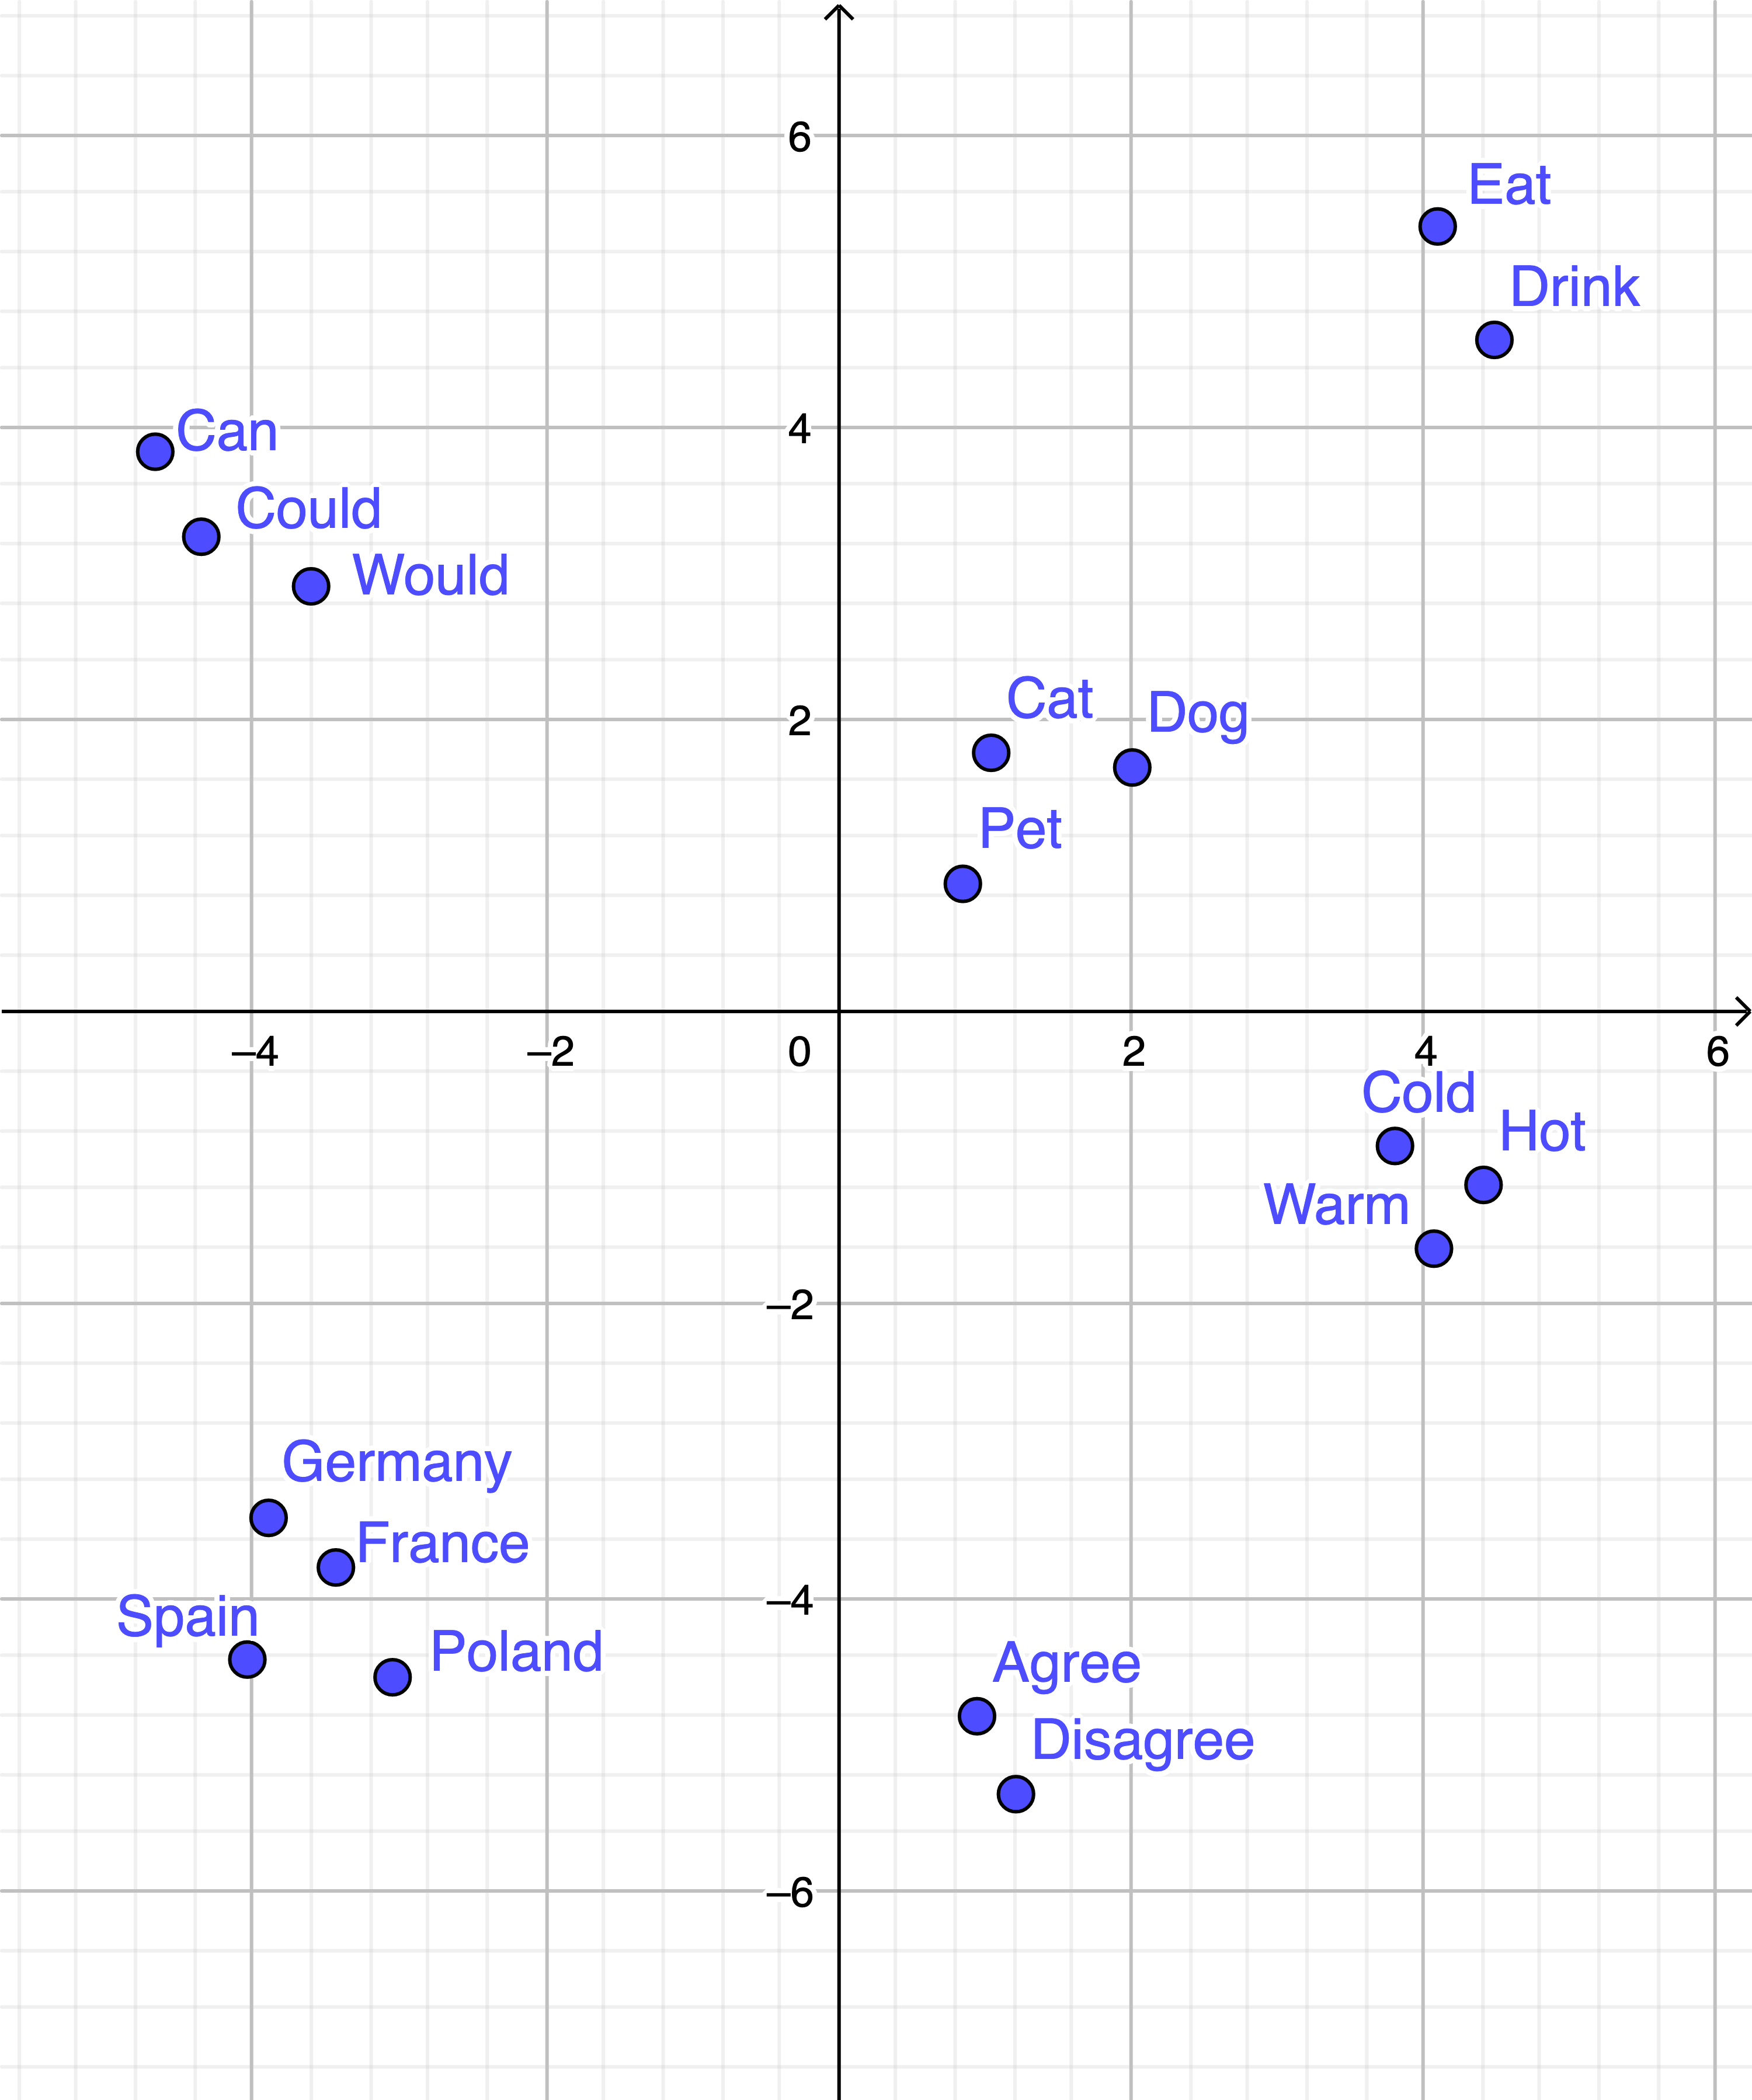
\includegraphics[width=4cm]{./figures/Groups}

	\end{figure}
		\begin{center}
		{Example result of word embedding}
		\end{center}
	\vspace{-0.5cm}

\end{frame}

%%%%%%%%%%%%%%%%%%%%%%%%%%%%%%%%%%%%%%%%%%%%%%%%%%%%%%%%%%%%%%%%%%%%%%%%%%%%%%%%%%%%%%%%%%%%%%%%%%%

%%%%%%%%%%%%%%%%%%%%%%%%%%%%%%%%%%%%%%%%%%%%%%%%%%%%%%%%%%%%%%%%%%%%%%%%%%%%%%%%%%%%%%%%%%%%%%%%%%%

\begin{frame}
	\frametitle{Word embedding}

	\begin{figure}
		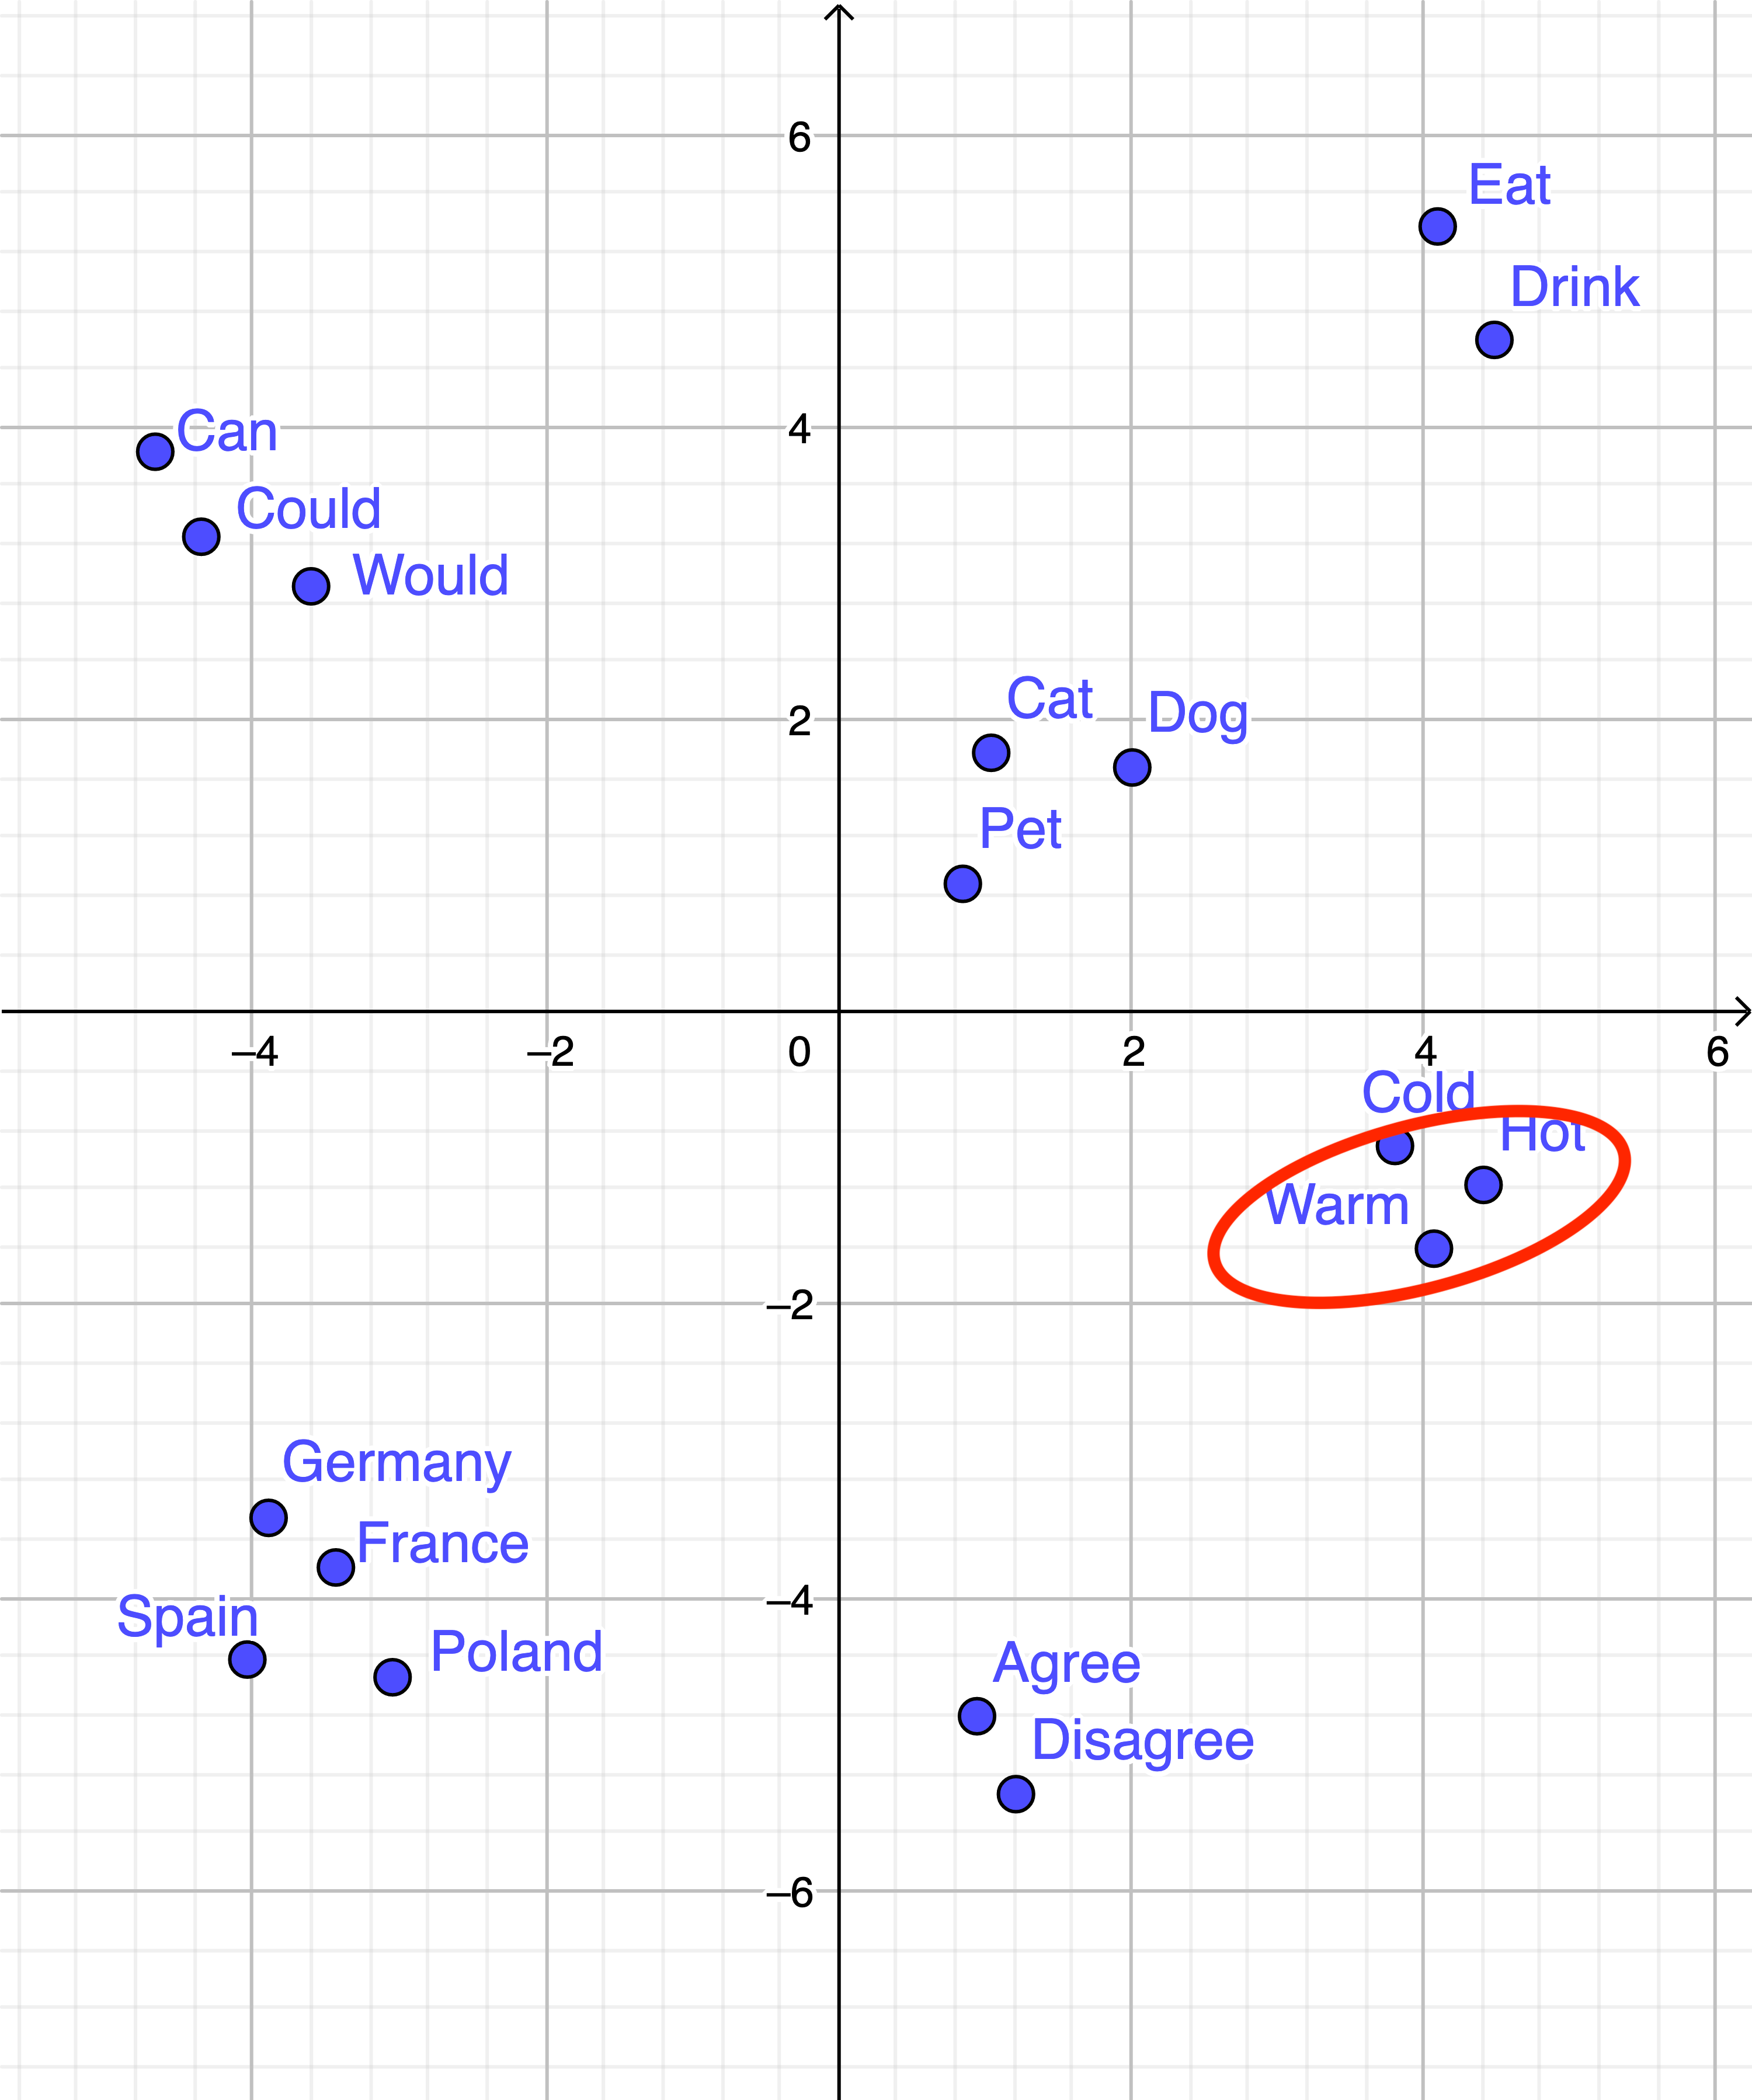
\includegraphics[width=4cm]{./figures/Group_synonym}

	\end{figure}
		\begin{center}
		{Words are synonyms}
		\end{center}
	\vspace{-0.5cm}

\end{frame}

%%%%%%%%%%%%%%%%%%%%%%%%%%%%%%%%%%%%%%%%%%%%%%%%%%%%%%%%%%%%%%%%%%%%%%%%%%%%%%%%%%%%%%%%%%%%%%%%%%%

%%%%%%%%%%%%%%%%%%%%%%%%%%%%%%%%%%%%%%%%%%%%%%%%%%%%%%%%%%%%%%%%%%%%%%%%%%%%%%%%%%%%%%%%%%%%%%%%%%%

\begin{frame}
	\frametitle{Word embedding}

	\begin{figure}
		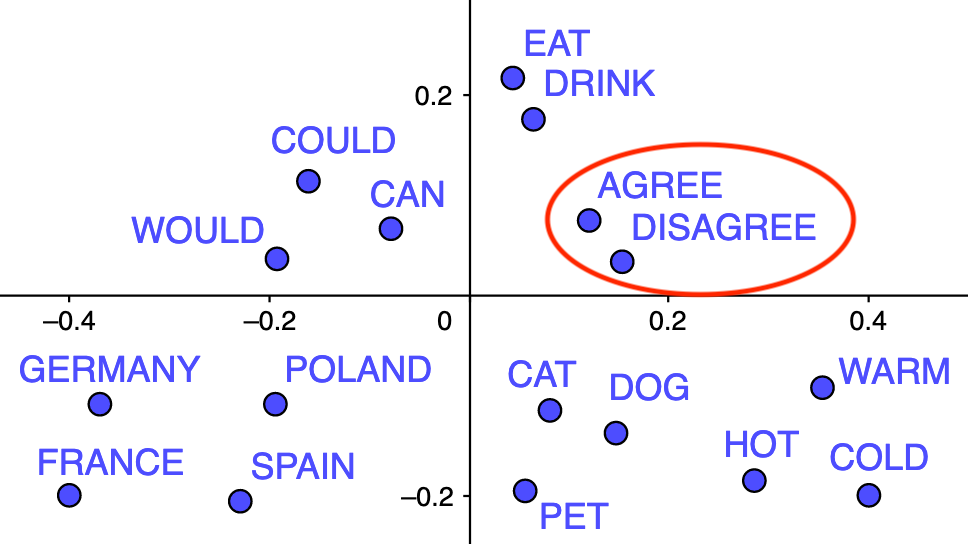
\includegraphics[width=4cm]{./figures/Group_antonyms}

	\end{figure}
		\begin{center}
		{Words are antonyms}
		\end{center}
	\vspace{-0.5cm}

\end{frame}

%%%%%%%%%%%%%%%%%%%%%%%%%%%%%%%%%%%%%%%%%%%%%%%%%%%%%%%%%%%%%%%%%%%%%%%%%%%%%%%%%%%%%%%%%%%%%%%%%%%

%%%%%%%%%%%%%%%%%%%%%%%%%%%%%%%%%%%%%%%%%%%%%%%%%%%%%%%%%%%%%%%%%%%%%%%%%%%%%%%%%%%%%%%%%%%%%%%%%%%

\begin{frame}
	\frametitle{Word embedding}

	\begin{figure}
		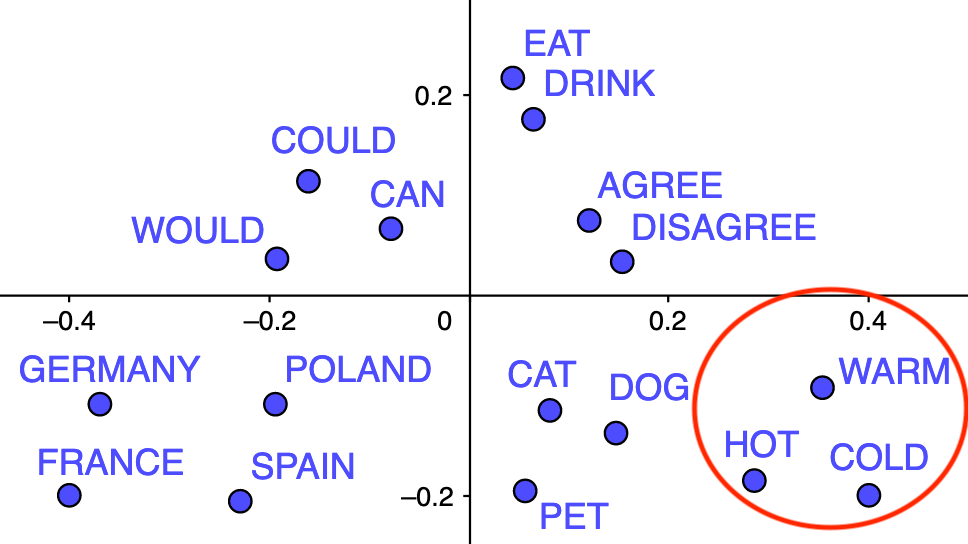
\includegraphics[width=4cm]{./figures/Group_scale}

	\end{figure}
		\begin{center}
		{Words are value on a scale}
		\end{center}
	\vspace{-0.5cm}

\end{frame}

%%%%%%%%%%%%%%%%%%%%%%%%%%%%%%%%%%%%%%%%%%%%%%%%%%%%%%%%%%%%%%%%%%%%%%%%%%%%%%%%%%%%%%%%%%%%%%%%%%%

%%%%%%%%%%%%%%%%%%%%%%%%%%%%%%%%%%%%%%%%%%%%%%%%%%%%%%%%%%%%%%%%%%%%%%%%%%%%%%%%%%%%%%%%%%%%%%%%%%%

\begin{frame}
	\frametitle{Word embedding}

	\begin{figure}
		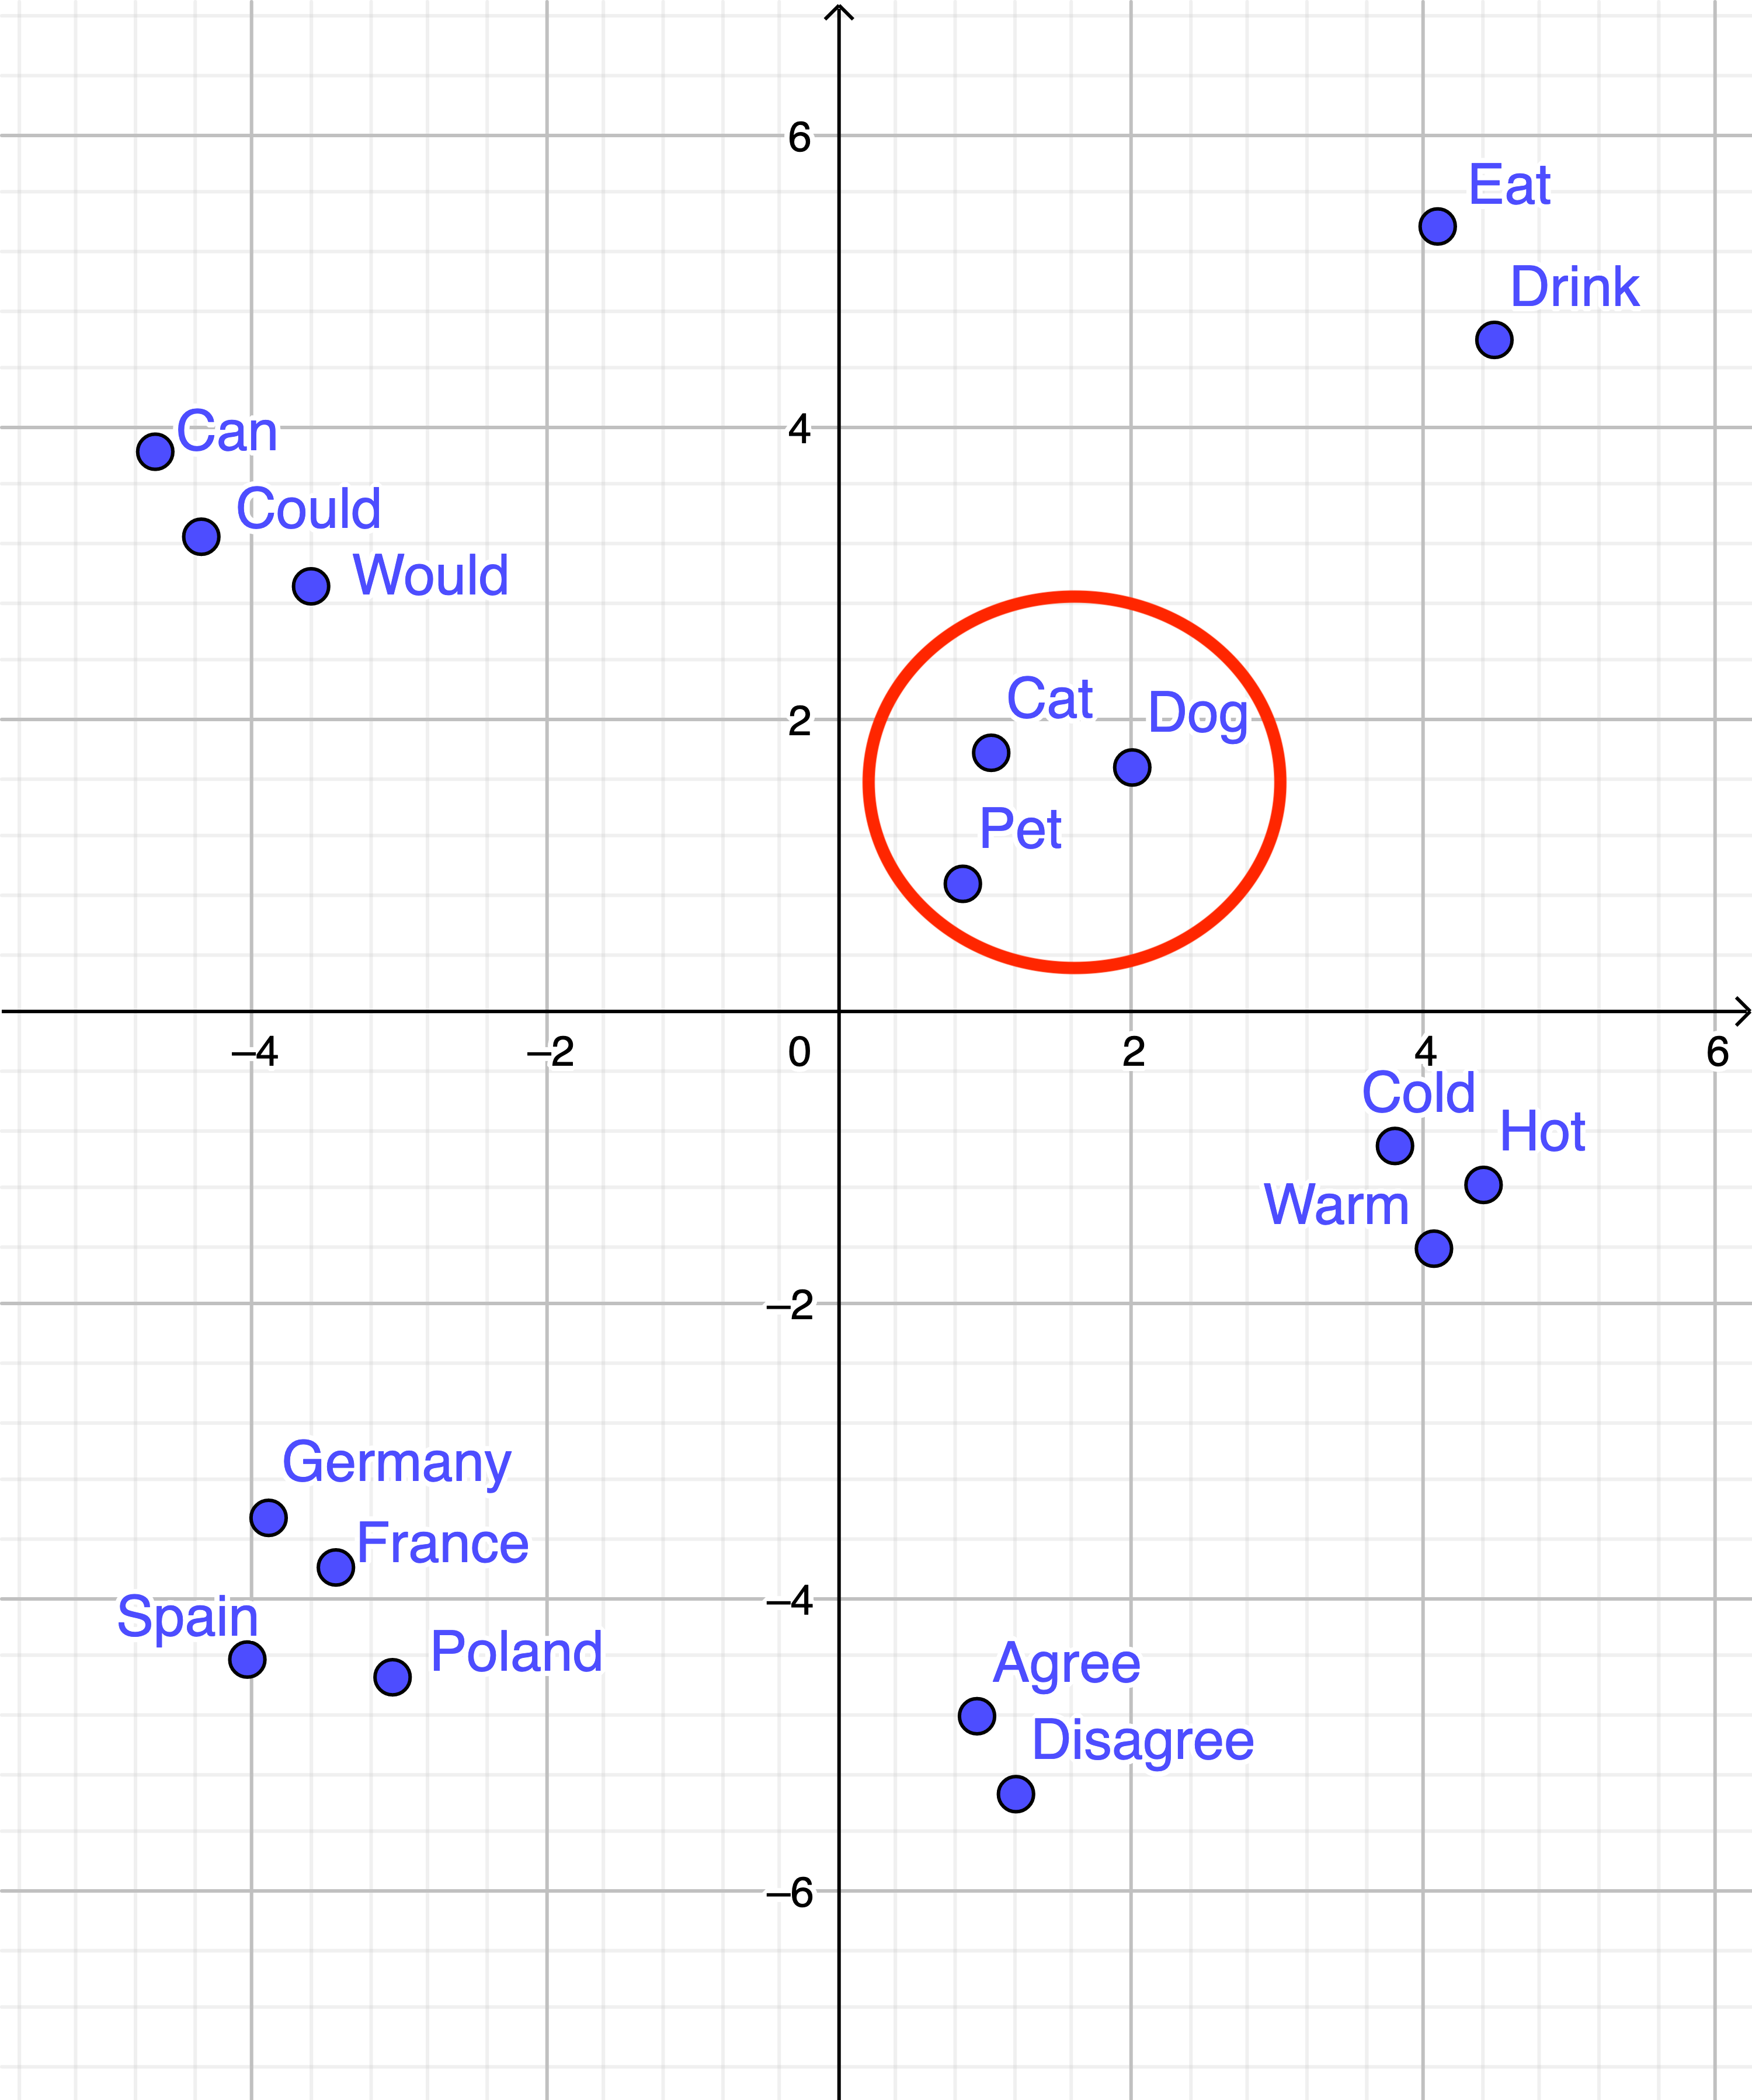
\includegraphics[width=4cm]{./figures/Group_hyponym}
	\end{figure}
		\begin{center}
		{Words are hyponym - hypernym}
		\end{center}
	\vspace{-0.5cm}

\end{frame}

%%%%%%%%%%%%%%%%%%%%%%%%%%%%%%%%%%%%%%%%%%%%%%%%%%%%%%%%%%%%%%%%%%%%%%%%%%%%%%%%%%%%%%%%%%%%%%%%%%%

%%%%%%%%%%%%%%%%%%%%%%%%%%%%%%%%%%%%%%%%%%%%%%%%%%%%%%%%%%%%%%%%%%%%%%%%%%%%%%%%%%%%%%%%%%%%%%%%%%%

\begin{frame}
	\frametitle{Word embedding}

	\begin{figure}
		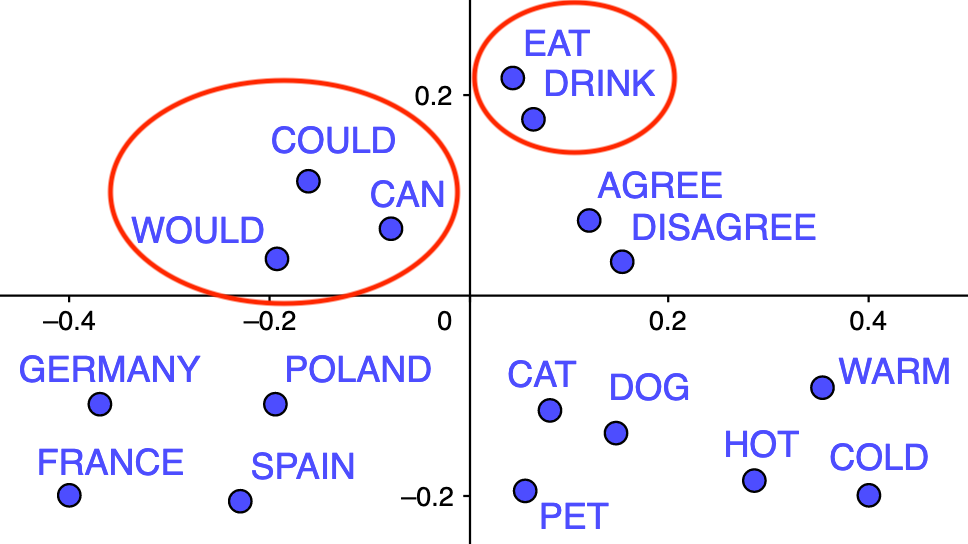
\includegraphics[width=4cm]{./figures/Group_context}
	\end{figure}
		\begin{center}
		{Words appear in similar context}
		\end{center}
	\vspace{-0.5cm}

\end{frame}

%%%%%%%%%%%%%%%%%%%%%%%%%%%%%%%%%%%%%%%%%%%%%%%%%%%%%%%%%%%%%%%%%%%%%%%%%%%%%%%%%%%%%%%%%%%%%%%%%%%

\section{Word embedding models}

%%%%%%%%%%%%%%%%%%%%%%%%%%%%%%%%%%%%%%%%%%%%%%%%%%%%%%%%%%%%%%%%%%%%%%%%%%%%%%%%%%%%%%%%%%%%%%%%%%%

\begin{frame}
\frametitle{Word embedding models}

	\begin{itemize}
		\item Training approaches
		\item Word2Vec
		\item GloVe
		\item FastText
	\end{itemize}

\end{frame}

\subsection{Training approaches}

%%%%%%%%%%%%%%%%%%%%%%%%%%%%%%%%%%%%%%%%%%%%%%%%%%%%%%%%%%%%%%%%%%%%%%%%%%%%%%%%%%%%%%%%%%%%%%%%%%%

\begin{frame}
\frametitle{How to train my embedding model?}
	
	\begin{itemize}
		\item CBOW
		\item Skip-gram
	\end{itemize}

\end{frame}

\begin{frame}
\frametitle{CBOW}
	\framesubtitle{Words representation}

	\begin{itemize}
		\item Continuous Bag-of-Words
		\item Prediction of current words based on context
		\item Context is determined by surrounding words
	\end{itemize}

\end{frame}

\begin{frame}
\frametitle{CBOW}
	\framesubtitle{Words representation}
%
	\begin{figure}
		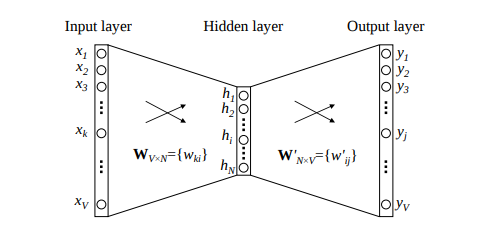
\includegraphics[width=8cm]{./figures/cbow_simple}
		\caption{Simple CBOW model with one word in the context}
	\end{figure}

\end{frame}


\begin{frame}
\frametitle{CBOW}
	\framesubtitle{Words representation}

%	\begin{center}
%		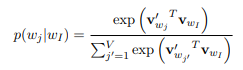
\includegraphics[width=6cm]{./figures/cbow_eq}
%	\end{center}

$$p(w_j|w_I)= \frac{\exp({v'_{w_j}}^{T}v_{w_I})}{ \sum_{j'=1}^{V} \exp({v'_{w_{j'}}}^{T}v_{w_I})}$$

\end{frame}


\begin{frame}
\frametitle{Skip-gram}
	\framesubtitle{Words representation}

	\begin{itemize}
		\item Continuous Skip-gram
		\item Predicting the surrounding words based on the context
		\item Context is the current word
	\end{itemize}

\end{frame}


\begin{frame}
\frametitle{CBOW vs Skip-gram}
	\framesubtitle{Words representation}

	\begin{figure}
		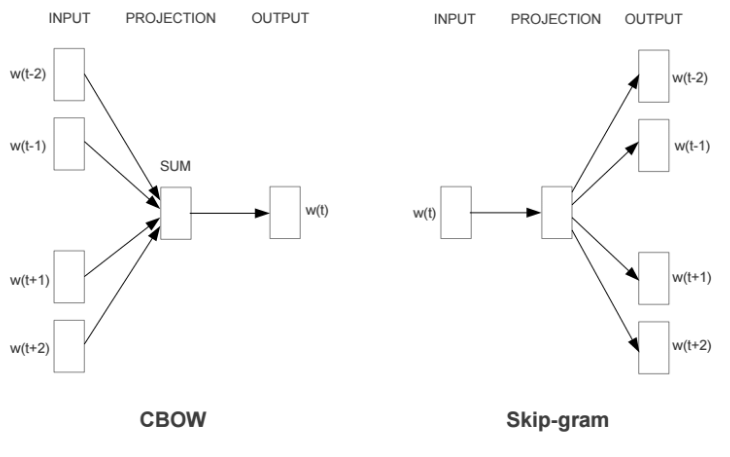
\includegraphics[width=6cm]{./figures/cbow_skip_gram}
		\caption{CBOW vs Skip-gram}
	\end{figure}
	
\end{frame}

%%%%%%%%%%%%%%%%%%%%%%%%%%%%%%%%%%%%%%%%%%%%%%%%%%%%%%%%%%%%%%%%%%%%%%%%%%%%%%%%%%%%%%%%%%%%%%%%%%%

\subsection{Word2Vec}

%%%%%%%%%%%%%%%%%%%%%%%%%%%%%%%%%%%%%%%%%%%%%%%%%%%%%%%%%%%%%%%%%%%%%%%%%%%%%%%%%%%%%%%%%%%%%%%%%%%

\begin{frame}
\frametitle{Word2Vec}
	\framesubtitle{Word embedding models}

	\begin{itemize}
		\item Created by researchers at Google in 2013
		\item Can use either CBOW or skip-gram
		\item Input is a corpus of text
		\item Produces vector space with unique word 
	\end{itemize}

\end{frame}

\begin{frame}
\frametitle{Word2Vec}
	\framesubtitle{Interesting parameters}

	\begin{itemize}
		\item Dimensionality!
		\item Training algorithm --- softmax vs negative sampling
		\item Context window
	\end{itemize}

\end{frame}

%%%%%%%%%%%%%%%%%%%%%%%%%%%%%%%%%%%%%%%%%%%%%%%%%%%%%%%%%%%%%%%%%%%%%%%%%%%%%%%%%%%%%%%%%%%%%%%%%%%

\subsection{GloVe}

%%%%%%%%%%%%%%%%%%%%%%%%%%%%%%%%%%%%%%%%%%%%%%%%%%%%%%%%%%%%%%%%%%%%%%%%%%%%%%%%%%%%%%%%%%%%%%%%%%%

\begin{frame}
\frametitle{GloVe}
	\framesubtitle{Word embedding models}

	\begin{itemize}
		\item Global Vectors for Word Representation
		\item Comes from Stanford University, open-source
		\item Kind of extension of Word2Vec
		\item Training performed on aggregated, global word-word co-occurence statistics
	\end{itemize}

\end{frame}

\begin{frame}
\frametitle{GloVe}
	\framesubtitle{Word embedding models}

	\begin{figure}
		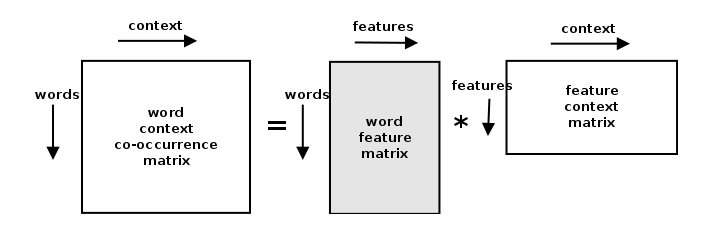
\includegraphics[width=9cm]{./figures/glove}
		\caption{Co-occurence statistics of words}
	\end{figure}

\end{frame}


%%%%%%%%%%%%%%%%%%%%%%%%%%%%%%%%%%%%%%%%%%%%%%%%%%%%%%%%%%%%%%%%%%%%%%%%%%%%%%%%%%%%%%%%%%%%%%%%%%%


\subsection{FastText}

%%%%%%%%%%%%%%%%%%%%%%%%%%%%%%%%%%%%%%%%%%%%%%%%%%%%%%%%%%%%%%%%%%%%%%%%%%%%%%%%%%%%%%%%%%%%%%%%%%%

\begin{frame}
\frametitle{FastText}
	\framesubtitle{Word embedding models}

	\begin{itemize}
		\item Incorporate sub-word information!
		\item Naturally support out-of-vocabulary words
		\item Uses skip-gram with negative sampling
	\end{itemize}

\end{frame}

\begin{frame}
\frametitle{FastText}
	\framesubtitle{Word embedding models}

	\begin{figure}
		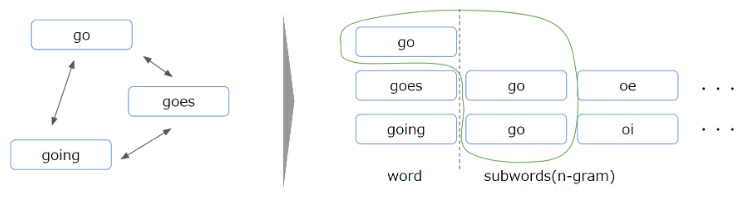
\includegraphics[width=9cm]{./figures/fasttext}
		\caption{FastText subwords example}
	\end{figure}

\end{frame}

%%%%%%%%%%%%%%%%%%%%%%%%%%%%%%%%%%%%%%%%%%%%%%%%%%%%%%%%%%%%%%%%%%%%%%%%%%%%%%%%%%%%%%%%%%%%%%%%%%%

\section{Applications}

%%%%%%%%%%%%%%%%%%%%%%%%%%%%%%%%%%%%%%%%%%%%%%%%%%%%%%%%%%%%%%%%%%%%%%%%%%%%%%%%%%%%%%%%%%%%%%%%%%%

\begin{frame}
\frametitle{}

\begin{center}
	\Huge {How can we use it?}
\end{center}
\end{frame}

%%%%%%%%%%%%%%%%%%%%%%%%%%%%%%%%%%%%%%%%%%%%%%%%%%%%%%%%%%%%%%%%%%%%%%%%%%%%%%%%%%%%%%%%%%%%%%%%%%%

\subsection{Natural Language Processing}

%%%%%%%%%%%%%%%%%%%%%%%%%%%%%%%%%%%%%%%%%%%%%%%%%%%%%%%%%%%%%%%%%%%%%%%%%%%%%%%%%%%%%%%%%%%%%%%%%%%

\begin{frame}
	\frametitle{Natural Language Processing}
	
	\begin{itemize}
		\item If user search for ``Dell notebook battery size'' we would like to match it also with ``Dell laptop battery capacity"
		\item If user search for ``Cracow Motel'' we would like to match it also with ``Krakow Hotel''
	\end{itemize}
	
\end{frame}

%%%%%%%%%%%%%%%%%%%%%%%%%%%%%%%%%%%%%%%%%%%%%%%%%%%%%%%%%%%%%%%%%%%%%%%%%%%%%%%%%%%%%%%%%%%%%%%%%%%

\begin{frame}
\frametitle{Natural Language Processing}

\begin{itemize}
	\item Analyzing survey responses
	\item Analyzing comments
\end{itemize}

\end{frame}

%%%%%%%%%%%%%%%%%%%%%%%%%%%%%%%%%%%%%%%%%%%%%%%%%%%%%%%%%%%%%%%%%%%%%%%%%%%%%%%%%%%%%%%%%%%%%%%%%%%

\subsection{Other domains}

%%%%%%%%%%%%%%%%%%%%%%%%%%%%%%%%%%%%%%%%%%%%%%%%%%%%%%%%%%%%%%%%%%%%%%%%%%%%%%%%%%%%%%%%%%%%%%%%%%%

\begin{frame}
\frametitle{Other domains}

\begin{itemize}
	\item Word2Vec can catch relationships and contexts in songs the user listens to
	\item Data can be used for real-time music recommendation
\end{itemize}

\end{frame}

%%%%%%%%%%%%%%%%%%%%%%%%%%%%%%%%%%%%%%%%%%%%%%%%%%%%%%%%%%%%%%%%%%%%%%%%%%%%%%%%%%%%%%%%%%%%%%%%%%%

\section{Problems and limitations}

%%%%%%%%%%%%%%%%%%%%%%%%%%%%%%%%%%%%%%%%%%%%%%%%%%%%%%%%%%%%%%%%%%%%%%%%%%%%%%%%%%%%%%%%%%%%%%%%%%%

\begin{frame}
\frametitle{Problems and limitations}

	\begin{itemize}
		\item Multiple meanings of a word: solution --- \textit{Sense} embeddings
		\item Inability to handle unknown or out-of-vocabulary (OOV) words
		\item Scaling to new languages
		\item No shared representations at sub-word levels
	\end{itemize}

\end{frame}

%%%%%%%%%%%%%%%%%%%%%%%%%%%%%%%%%%%%%%%%%%%%%%%%%%%%%%%%%%%%%%%%%%%%%%%%%%%%%%%%%%%%%%%%%%%%%%%%%%%

\section{Summary}

%%%%%%%%%%%%%%%%%%%%%%%%%%%%%%%%%%%%%%%%%%%%%%%%%%%%%%%%%%%%%%%%%%%%%%%%%%%%%%%%%%%%%%%%%%%%%%%%%%%

\begin{frame}
	\frametitle{}
	
	\begin{center}
		\Huge {Summary}
	\end{center}
\end{frame}

%%%%%%%%%%%%%%%%%%%%%%%%%%%%%%%%%%%%%%%%%%%%%%%%%%%%%%%%%%%%%%%%%%%%%%%%%%%%%%%%%%%%%%%%%%%%%%%%%%%

\begin{frame}
	\frametitle{Summary}
	
	\begin{itemize}
		\item ...
		\item ...
	\end{itemize}
	
\end{frame}

%%%%%%%%%%%%%%%%%%%%%%%%%%%%%%%%%%%%%%%%%%%%%%%%%%%%%%%%%%%%%%%%%%%%%%%%%%%%%%%%%%%%%%%%%%%%%%%%%%%
\begin{frame}

\begin{center}
	\Huge \textbf{Thank you for your attention!}
\end{center}

\end{frame}
%%%%%%%%%%%%%%%%%%%%%%%%%%%%%%%%%%%%%%%%%%%%%%%%%%%%%%%%%%%%%%%%%%%%%%%%%%%%%%%%%%%%%%%%%%%%%%%%%%%

%%%%%%%%%%%%%%%%%%%%%%%%%%%%%%%%%%%%%%%%%%%%%%%%%%%%%%%%%%%%%%%%%%%%%%%%%%%%%%%%%%%%%%%%%%%%%%%%%%%
\begin{frame}

\begin{center}
\Huge \textbf{Q \& A}
\end{center}

\end{frame}
%%%%%%%%%%%%%%%%%%%%%%%%%%%%%%%%%%%%%%%%%%%%%%%%%%%%%%%%%%%%%%%%%%%%%%%%%%%%%%%%%%%%%%%%%%%%%%%%%%%

\begin{frame}[allowframebreaks]
\frametitle{References}
%\bibliographystyle{plain}
\nocite{*}
\setbeamertemplate{bibliography item}[online]
\bibliography{bibliographyfile}
\bibliographystyle{plain}
\nocite{*}
\setbeamertemplate{bibliography item}[online]
\bibliography{bibliographyfile}
\end{frame}

%%%%%%%%%%%%%%%%%%%%%%%%%%%%%%%%%%%%%%%%%%%%%%%%%%%%%%%%%%%%%%%%%%%%%%%%%%%%%%%%%%%%%%%%%%%%%%%%%%%









%%%%%%%%%%%%%%%%%%%%%%%%%%%%%%%%%%%%%%%%%%%%%%%%%%%%%%%%%%%%%%%%%%%%%%%%%%%%%%%%%%%%%%%%%%%%%%%%%%%
%\begin{frame}
%	\frametitle{Title of the Slide}
%		\framesubtitle{Subtitle of the Slide: Use Only if Necessary\dots}
%	
%	\begin{itemize}
%		\item Bulalet point 1.
%		\item Bullet point 2 -e-- \alert{you can emphasise} a text.
%	\end{itemize}
%
%\end{frame}
%
%%%%%%%%%%%%%%%%%%%%%%%%%%%%%%%%%%%%%%%%%%%%%%%%%%%%%%%%%%%%%%%%%%%%%%%%%%%%%%%%%%%%%%%%%%%%%%%%%%%%
%\begin{frame}
%	\frametitle{Title of the Slide}
%		\framesubtitle{Slide without Bullets}
%
%	Text:
%
%	\vfill
%
%	\begin{block}{}
%		Blocks are good for important notions.
%	\end{block}
%
%	\vfill
%
%	\begin{alertblock}{}
%		Alertblocks are even better to catch the attention.
%	\end{alertblock}
%
%	\vfill
%
%	\begin{alertblock}{Title}
%		You can have the title in the (alert)block.
%	\end{alertblock}
%
%\end{frame}
%
%%%%%%%%%%%%%%%%%%%%%%%%%%%%%%%%%%%%%%%%%%%%%%%%%%%%%%%%%%%%%%%%%%%%%%%%%%%%%%%%%%%%%%%%%%%%%%%%%%%%
%\begin{frame}
%	\frametitle{Title of the Slide}
%		\framesubtitle{Slide with a Figure from a File}
%
%	\begin{figure}
%		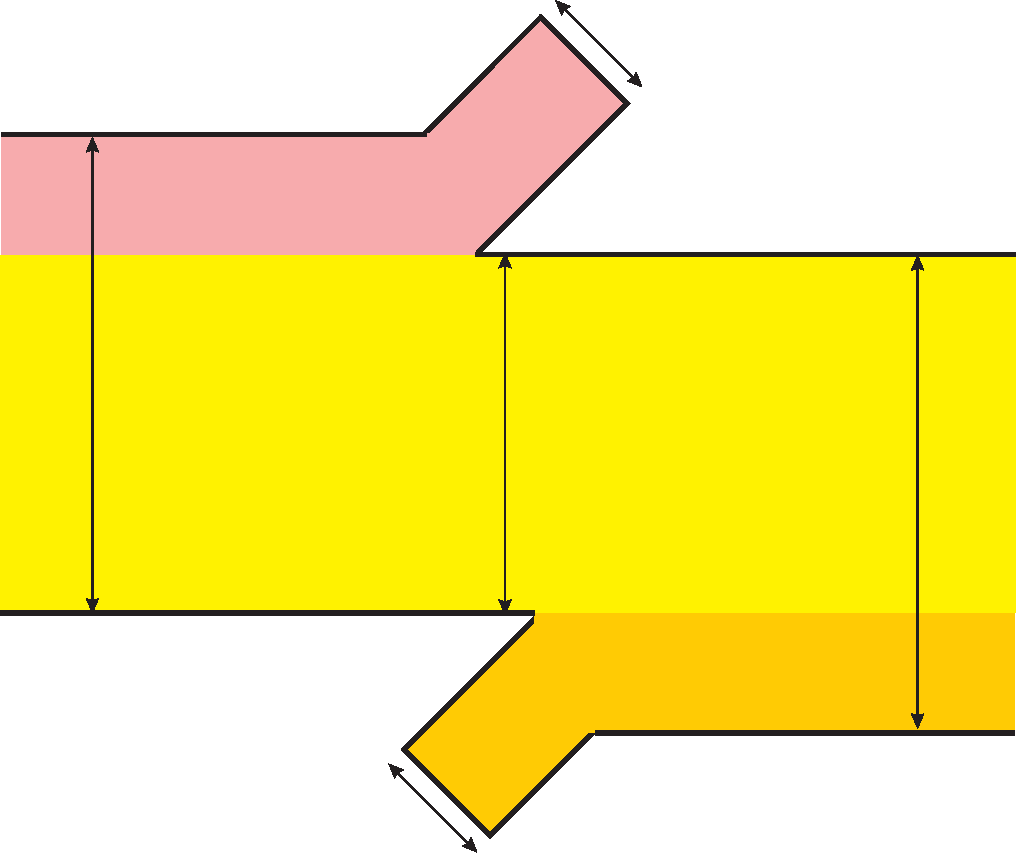
\includegraphics[width=6cm]{./figures/TIiK_channel_mutual_new}
%		\caption{Caption of the figure}
%	\end{figure}
%
%	\vspace{-0.5cm}
%
%	\tiny I am sorry that the example figures and the table concern the information theory \smiley
%
%\end{frame}
%%%%%%%%%%%%%%%%%%%%%%%%%%%%%%%%%%%%%%%%%%%%%%%%%%%%%%%%%%%%%%%%%%%%%%%%%%%%%%%%%%%%%%%%%%%%%%%%%%%%
%
%%%%%%%%%%%%%%%%%%%%%%%%%%%%%%%%%%%%%%%%%%%%%%%%%%%%%%%%%%%%%%%%%%%%%%%%%%%%%%%%%%%%%%%%%%%%%%%%%%%%
%\begin{frame}
%	\frametitle{Title of the Slide}
%		\framesubtitle{Slide with a Figure Drawn with \texttt{tikz}}
%
%	\vspace{-0.5cm}
%
%	\begin{changemargin}{-1cm}{-1cm}
%		\begin{figure}
%			\begin{tikzpicture}[x=2.5cm,y=2cm]
%				\node[draw,thick,rectangle,fill=blue!25,align=center,text width = 1.5cm] (SOURCE) at (0,0) {\bfseries Source}; 
%				\node[draw,thick,rectangle,fill=green!25,label=above:{\it Compression},align=center,text width = 1.5cm] (SOURCE_ENCODER) at (1,0) {\bfseries Source encoder}; 
%				\node[draw,thick,rectangle,fill=magenta!25,label=above:{\it Security},align=center,text width = 2.00cm] (ENCRYPTION) at (2,0) {\bfseries Encryption}; 
%				\node[draw,thick,rectangle,fill=red!25,align=center,text width = 1.5cm] (CHANNEL_ENCODER) at (3,0) {\bfseries Channel encoder};
%				\node[align=center,text width = 1.5cm,yshift=1.05cm] at (CHANNEL_ENCODER) {\it Error\\protection}; 
%				\node[draw,thick,rectangle,fill=gray!25,align=center,text width = 2.25cm] (MODULATOR) at (4,0) {\bfseries Modulator}; 
%				\node[draw,thick,rectangle,fill=yellow!25,align=center,text width = 1.5cm] (CHANNEL) at (4,-1) {\bfseries Channel}; 
%				\node[draw,thick,rectangle,fill=gray!25,align=center,text width = 2.25cm] (DEMODULATOR) at (4,-2) {\bfseries Demodulator}; 
%				\node[draw,thick,rectangle,fill=red!25,align=center,text width = 1.5cm] (CHANNEL_DECODER) at (3,-2) {\bfseries Channel decoder}; 
%				\node[draw,thick,rectangle,fill=magenta!25,align=center,text width = 2.00cm] (DECRYPTION) at (2,-2) {\bfseries Decryption}; 
%				\node[draw,thick,rectangle,fill=green!25,align=center,text width = 1.5cm] (SOURCE_DECODER) at (1,-2) {\bfseries Source decoder}; 
%				\node[draw,thick,rectangle,fill=blue!25,align=center,text width = 1.5cm] (SINK) at (0,-2) {\bfseries Sink}; 
%				\node[starburst, fill=yellow, draw=red,line width=1pt,shift={(0.25,0.60cm)}] (NOISE) at (CHANNEL) {\color{red} \bf \tiny !};
%	% 			\node[align=center,text width = 1.5cm] at (NOISE) {\color{red} Noise,\\errors,\\frauds};
%				\draw[thick,->] (SOURCE) -- (SOURCE_ENCODER) ;
%				\draw[thick,->] (SOURCE_ENCODER) -- (ENCRYPTION);
%				\draw[thick,->] (ENCRYPTION) -- (CHANNEL_ENCODER);
%				\draw[thick,->] (CHANNEL_ENCODER) -- (MODULATOR);
%				\draw[thick,->] (MODULATOR) -- (CHANNEL);
%				\draw[thick,->] (CHANNEL) -- (DEMODULATOR);
%				\draw[thick,->] (DEMODULATOR) -- (CHANNEL_DECODER);
%				\draw[thick,->] (CHANNEL_DECODER) -- (DECRYPTION);
%				\draw[thick,->] (DECRYPTION) -- (SOURCE_DECODER);
%				\draw[thick,->] (SOURCE_DECODER) -- (SINK);
%				\coordinate (c1) at ($(CHANNEL_DECODER.south) + (0,-0.25cm)$);
%				\draw[thick] (CHANNEL_DECODER) -- (c1);
%				\draw[thick,->] (c1) -| (DEMODULATOR.south);
%				\node at (3.5,-2.5) {\it Iterative decoding};
%				\node[align=center,text width = 1.5cm] (SCT) at (1,-1) {Source\\coding\\theorem};
%				\draw[->] (SCT) -- +(0,1.25cm);
%				\draw[->] (SCT) -- +(0,-1.25cm);
%				\node[align=center,text width = 1.5cm] (CCT) at (3,-1) {Channel\\coding\\theorem};
%				\draw[->] (CCT) -- +(0,1.25cm);
%				\draw[->] (CCT) -- +(0,-1.25cm);
%				\draw[->] (CCT) -- +(0.5,0cm);
%			\end{tikzpicture}
%		\end{figure}		
%	\end{changemargin}
%
%	\vspace{-0.35cm}
%
%	\tiny Source: \bibentry{Moon05a}.
%
%\end{frame}
%%%%%%%%%%%%%%%%%%%%%%%%%%%%%%%%%%%%%%%%%%%%%%%%%%%%%%%%%%%%%%%%%%%%%%%%%%%%%%%%%%%%%%%%%%%%%%%%%%%%
%
%%%%%%%%%%%%%%%%%%%%%%%%%%%%%%%%%%%%%%%%%%%%%%%%%%%%%%%%%%%%%%%%%%%%%%%%%%%%%%%%%%%%%%%%%%%%%%%%%%%%
%\begin{frame}
%	\frametitle{Title of the Slide}
%		\framesubtitle{Slide with a Table}
%	
%		\begin{table}
%			\caption{Caption of the Table}
%			\begin{center}
%				\setlength\arrayrulewidth{2pt}
%					\begin{tabular}{|>{\columncolor[rgb]{0,0.9,0.3}\color{white}}c|>{\columncolor[rgb]{0,0.9,0.1}\color{white}}c|}
%					\hline
%					\rowcolor[rgb]{0,0.5,0} \bfseries Data  & \bfseries Entropy \\
%					\hline%
%					\hline Plain text                        	  & $4{.}347$\\
%					\hline Native executables	                   & $5{.}099$\\
%					\hline Packed executables                   & $6{.}801$\\
%					\hline Encrypted executables                & $7{.}175$\\
%					\hline
%				\end{tabular}
%			\end{center}
%		\end{table}
%
%		\vfill
%
%		\tiny Source: \bibentry{Lyda07a}.
%\end{frame}
%%%%%%%%%%%%%%%%%%%%%%%%%%%%%%%%%%%%%%%%%%%%%%%%%%%%%%%%%%%%%%%%%%%%%%%%%%%%%%%%%%%%%%%%%%%%%%%%%%%